\setcounter{section}{0}
\section{Introduction}
This lab handbook serves as a side-by-side reference manual for you to use in your laboratory sessions. Not all information is included here (we expect you do to some research of your own) but it is a good starting point. It also includes some additional information you may find useful as you use the Raspberry Pi.

This handbook covers a range of topics from installation, to networking, to some more advanced topics such as cross compilation. There are links to useful learning resources, as well as some quick reference guides for you to refer back to as you work through all your practicals.

\section{Setting up your Pi}
In order to use the Pi you need to install an operating system on it and setup its networking.  The following will lead you through installing Raspbian as an operating system.  Raspbian  is a fork of the Debian distribution of the open source operating system Linux.  You will then configure the networking settings in Raspbian to allow you to access the Pi remotely using SSH.  

It is assumed that the user is running Windows, but the process will be similar for users of any operating system. It is recommended that during this course users gain familiarity with a Linux based OS such as Ubuntu

\subsection{Prerequisites}
\label{sec:Prereqs}
Download the following software applications and install them as indicated on their webpages
\textbf{TODO: These resources are also available on Vula.}
\begin{itemize}
    \item Latest Rasbian Stretch with Desktop and Recommended Software image, available at\\ \href{https://www.raspberrypi.org/downloads/raspbian}{Raspberry Pi Foundation Website}
    \item PuTTY (the full suite) available at\\ \href{https://www.chiark.greenend.org.uk/~sgtatham/putty/latest.html}{https://www.chiark.greenend.org.uk/~sgtatham/putty/latest.html}. \footnote{Some versions of Windows have the required SSH and SCP packages, but PuTTY has many other tools that are useful.}
    \item SDFormatter, available at\\ \href{https://www.sdcard.org/downloads/formatter_4/eula_windows/index.html}{https://www.sdcard.org/downloads/formatter\_4/eula\_windows/index.html}
    \item Etcher, an image writing tool, available at\\
    \href{https://www.balena.io/etcher/}{https://www.balena.io/etcher/}
\end{itemize}

\subsection{Install and configure Raspbian}
\begin{enumerate}
    \item Insert the SD card into the computer. If you do not have a reader available, speak to a friend or tutor who does.
    \item Write image to SD card\\
        Open Etcher. Select the downloaded zip image, and the SD card, and format. At the end of format, it may read that it failed,  but don't worry. Upon completion, Windows will try to mount partitions on the SD card that it can't read. Just press "Cancel" and then "OK" to the dialog boxes that pop up. The boot partition is the only partition we will be dealing with.
    \item Boot\\
    Insert SDCard into Pi and Plugin a screen and keyboard. If you do not have a keyboard, mouse and screen available, refer to the headless installation below.
    \item Configure\\
    For practicals you will need to enable a few services on the Pi.
    \begin{itemize}
        \item Open a terminal. You can either click the icon or press Ctrl+Alt+T
        \item Run \$ sudo raspi-config
        \item Scroll down to "interfacing Options"
        \item Enable SSH, VNC, SPI, I2C and Serial
    \end{itemize}
\end{enumerate}

\subsection{Headless Installation}
Headless mode on the Raspberry Pi refers to using it without direct user input and output (essentially no screen, mouse or keyboard connected directly to it). This is how all of the practicals will be conducted, as it is how most IoT devices are configured (over a network).

To use the RPi in headless mode, you at least need to enable SSH. Refer to Section \ref{sec:SSH} for instructions on how to do so. Once you have enabled SSH, be sure to run \$sudo raspi-config and enable VNC, SPI, I2C and Serial.

\subsection{Testing}
Once you've completed the installation process, including all relevant network configurations and SSH, be sure to test your connection and configuration before the first lab by logging in to the Pi through SSH or VNC.
% Bash
\section{The Unix Shell}
\label{app:UsefulResources}
Being able to use the Unix Shell and terminal commands is an invaluable skill, and a requirement for this course. Follow \href{https://swcarpentry.github.io/shell-novice/}{this guide} (https://swcarpentry.github.io/shell-novice/) for learning resources.

Some useful commands include:
\begin{table}[H]
\centering
\caption{Some useful shell commands}
\label{tbl:commands}
\begin{tabular}{|l|l|}
\hline
\textbf{Command} & \textbf{Use} \\ \hline
ls & \begin{tabular}[c]{@{}l@{}}List current files and folders in directory.\\ ls -al is useful to list everything\end{tabular} \\ \hline
cd \textless{}directory\textgreater{} & \begin{tabular}[c]{@{}l@{}}Change to a specified directory.\\ eg "cd .. " will take you one level up\end{tabular} \\ \hline
ifconfig & Shows current network interfaces and how they are connected \\ \hline
touch \textless{}file\textgreater{} & create \textless{}file\textgreater{} \\ \hline
nano \textless{}file\textgreater{} & Opens \textless{}file\textgreater in the nano text editor \\ \hline
vim \textless{}file\textgreater{} & Opens \textless{}file\textgreater in the vim text editor \\ \hline
mkdir \textless{}dir\textgreater{} & Creates the folder specified in \textless{}dir\textgreater{} \\ \hline
sudo \textless{}cmd\textgreater{} & executes the command \textless{}cmd\textgreater as an administrator \\ \hline
raspi-config &  \begin{tabular}[c]{@{}l@{}}Must be run as administrator\\ Opens up the Raspberry Pi Configuration Tool\end{tabular} \\ \hline
TODO & TODO \\ \hline
\end{tabular}
\end{table}


\section{The Raspberry Pi Pinout}
This course uses the Raspberry Pi 3B+. The pinout for this device is shown below. Note that some pins have special uses. This pins may not be able to be used as GPIO. Note that the header has a notch to indicate pin 1.  

\begin{figure}[H]
\centering
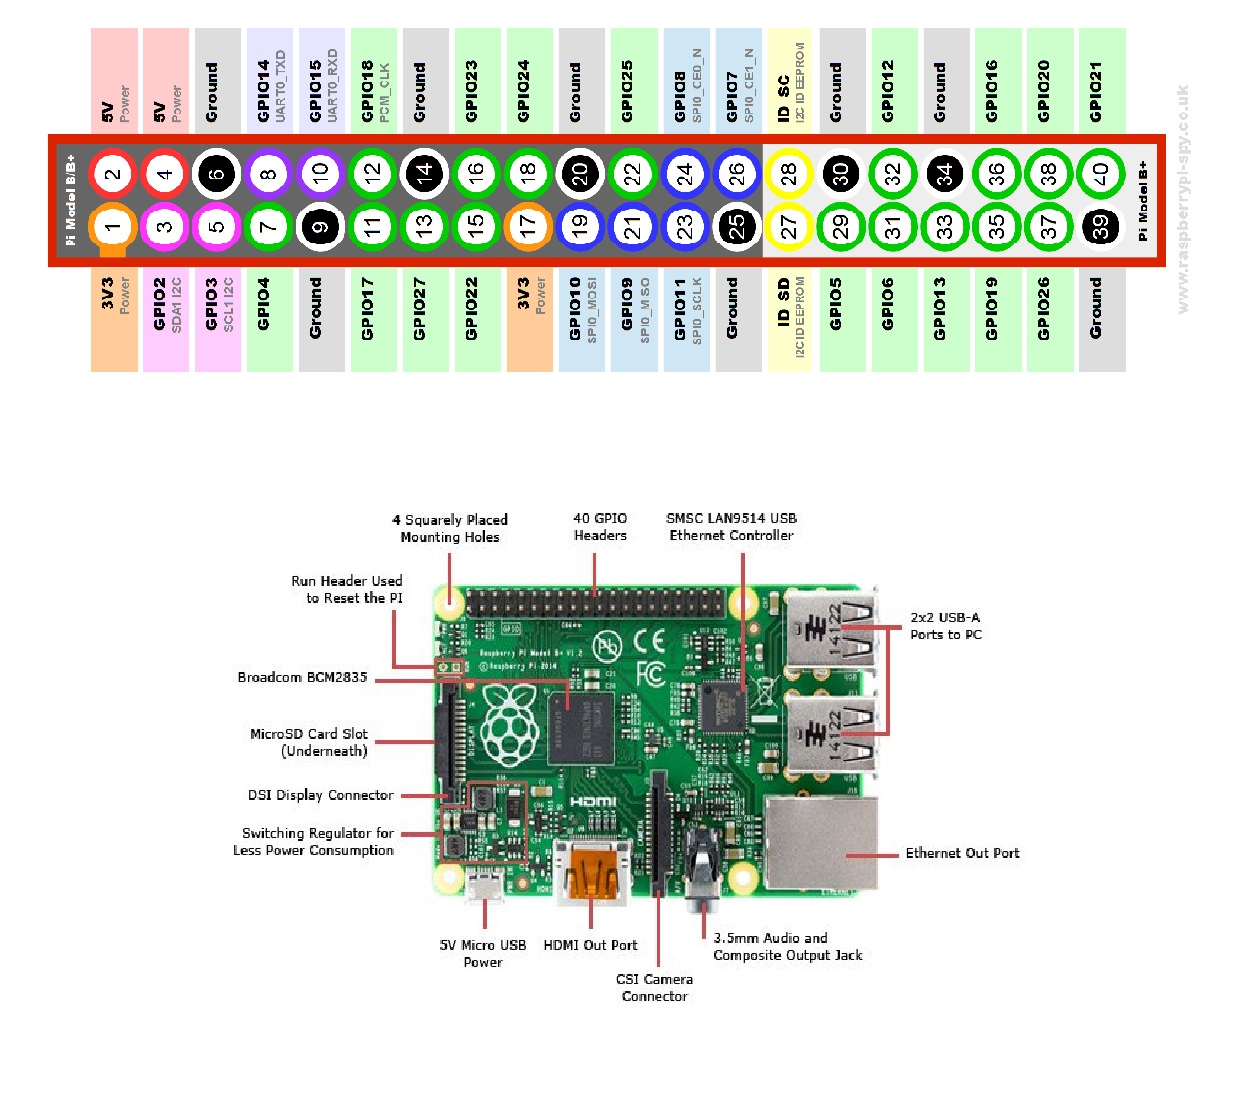
\includegraphics[width=1\columnwidth]{Figures/pinout}
\caption{GPIO Header of the B+ \href{https://www.jameco.com/Jameco/workshop/circuitnotes/raspberry-pi-circuit-note.html}{(source)}}
\label{fig:pinout}
\end{figure}



% Git
\section{Git}
\label{sec:Git}
Throughout the course you will be required to write and submit code and other files to an online git repository.  Git is a popular version control application that allows you to keep a record of changes you have made to text based files over time.  Additionally, by using a version controlled repository that is accessible to other collaborators, it provides a powerful way for many people to collectively build a larger system.  Almost all open source projects use a version control system to enable them to work with anyone else around the world in a structured and organised manner.  There are many platforms that offer free hosting services where you are able to share repositories, Github, and Gitlab are 2 such options.  Making an account on either of these (or a similar alternative) allows you to: (1) keep track of your own projects and the changes you make to them, (2) work collaboratively with team mates if you choose to share your repositories with them, and (3) is an increasingly common way of sharing a portfolio of your prior work with potential employers.

Git is a local tool. To use online backups, it's recommended to use a remote (online) repository management tool. GitHub is recommended because, as a student, there are many benefits which you can access. See \href{https://education.github.com/pack}{https://education.github.com/pack} for signing up.

Git can be intimidating in the beginning, but it becomes invaluable as you progress in software development. \href{https://swcarpentry.github.io/git-novice/}{This page} has a great guide you can follow to get well acquainted.

Before arriving at Prac 1, make sure you have created a demo repository on a computer and pushed it to the cloud using the instructions found below.

\subsection{A Quick Git Get Go}
\subsubsection{Creating a GitHub account and configuring your computer appropriately}
\begin{itemize}
    \item Start by creating a GitHub account
    \item Install git on your computer\\
    Lab computers already have git installed.\\
    If you're using a linux based system, this can be as simple as \verb|sudo apt-get install git|\\
    If you're using Windows, you need to download and use an installer.
    \item Once git is installed, run the following commands:\\
    Note: Do not do this on the lab computers. If you are on a lab computer, rather set the user.name and user.email parameters from within the created git repository, and do not use the \--\--global flag.\\
    git config \--\--global user.name "Your Name"\\
    git config \--\--global user.email "github email address"
    \item Git is now configured
\end{itemize}

\subsubsection{Creating a New Project}
Git consists of three primary stages: Untracked, staged and committed. Untracked files are not tracked by the repository. Staged files are files staged for commit but not yet committed. Committed files are "saved" to git.
On your local system:
\begin{itemize}
    \item Create a folder and enter into it
    \item Run \verb|git init|
    \item Create a new text file, for example "test.txt"
    \item Run \verb|git status|
    \item You will see there is an untracked file. Add it to git by running \verb|git add test.txt|
    \item It is possible to add all untracked files by running \verb|git add .|
    \item If you run \verb|git status| again, you will see that "test.txt" has been staged, but not yet committed. Commit test.txt by running \verb|git commit -m "Created test.txt"|. The \verb|-m| flag is to include a git commit message. It's useful to use these messages to explain what has changed in this commit.
\end{itemize}

\subsubsection{Linking GitHub and your Local Project}
On GitHub, create a new repository and give it a meaningful name and description. Take note of the link (something like https://github.com/\textless username\textgreater /\textless project-name\textgreater .git)

GitHub gives instructions on how to push an existing repository from the command line, but for completeness sake the commands are included here:
\begin{verbatim}
git remote add origin https://github.com/<username>/<project-name>.git
git push -u origin master    
\end{verbatim}

If you refresh the GitHub page, you should now see your files and commits.

\subsubsection{Understanding .gitignore}
Related SW Carpentry link: \href{https://swcarpentry.github.io/git-novice/06-ignore/index.html}{Ignoring Things}

You may have seen the option to add a .gitginore when creating a new repository on GitHub. This is used to get Git to ignore certain files, such as interim or raw data files. 
\section{\LaTeX}
\LaTeX is a great way to write documents, and is required for use in all your documents to be submitted for this course. \LaTeX is better than basic text editors such as Microsoft Word or Google Docs due to the following\footnote{Adapted from \href{https://academia.stackexchange.com/questions/5414/what-are-the-advantages-or-disadvantages-of-using-latex-for-writing-scientific-p}{this stack exchange question}}:
\begin{itemize}
    \item Dealing with mathematical notation.\\
    Layout and entry are generally easier using LaTeX than some other sort of equation editor. Online tools such as \href{http://detexify.kirelabs.org/classify.html}{Detexify} make it very simple to find the symbol you need.
    \item Consistent handling of intra-document references and bibliography.\\
    As of a couple of years ago the major editors still had problems with re-numbering cross-references and bibliography items. This is never a problem with BibTeX or LaTeX.
    \item Separation of content and style.\\
    In principle this means that you can write your document without caring how it is formatted, and at the end of the day wrap it in the style-file provided by the journal publisher before submission to conform to the house style. In practice some of the journal publishers demand special formatting commands that partially moots this process. Furthermore recent versions of Word and LibreOffice Writer, when properly used, should be able to keep track of various levels of section heading separate from the body text, and apply uniform styling to each level. The gap is somewhat closing.
    \item Tables and illustrations.\\
    With online tools such as \href{https://www.tablesgenerator.com/}{Tables Generator}, creating tables in \LaTeX is as simple as copy-pasting data from excel. Images can be inserted exactly where you specify them without worrying about justification or overlay.
\end{itemize}

There are a few difficulties with \LaTeX. These include difficulties with collaborative editing (consider the convenience of Google Docs), spell check (Microsoft Word has a much more advanced spell and grammar check) and ease of use (\LaTeX is technically a "document preparation system" as opposed to a text editor). However, many of these issues are mitigated by the use of an online tool known as \href{https://www.overleaf.com}{Overleaf}. Overleaf provides you with templates, the ability to collaborate, and (thankfully), a spell check function. It runs in browser and doesn't require any installation. If you would like to run an offline version, there are various options, but I suggest using Visual Studio Code with the \href{https://github.com/James-Yu/LaTeX-Workshop/wiki/Install}{Latex Workshop Plugin}.
\section{Networking on the Pi}
\subsection{A Brief Overview of Networks}
\label{app:UnderstandingNetworks}
It is useful to have a basic idea of how networks, IP addresses, and subnets work. For this, it it suggested you read \href{https://support.microsoft.com/en-za/help/164015/understanding-tcp-ip-addressing-and-subnetting-basics}{this article} from Microsoft: \href{https://tinyurl.com/y2z8x9za}{https://tinyurl.com/y2z8x9za}

\label{app:NetworkingOnThePi}
There are many ways to interface with the Pi. This section will cover types of network connectivity.

\subsection{Ethernet}
\label{sec:Connectivity-Ethernet}
This section will assign a static Ethernet address to the Raspberry Pi. This is useful for your first configuration.
\begin{enumerate}
    \item Insert the SD card into your computer and navigate to the BOOT partition
    \item open "cmdline.txt" and append the following to the line (don't create a new line)
        \begin{verbatim}ip=192.168.137.15\end{verbatim} 
        This tells the Raspberry Pi to configure the Ethernet port to use the IP address 192.168.137.15
    \item Enable SSH as per Section \ref{sec:SSH}
    \item You need to configure your PC to use the same subnet as the Pi. To do so, see Section \ref{sec:Connectivity-ChangeComputerIP}
\end{enumerate}

\subsection{Changing the IP on your computer}
\label{sec:Connectivity-ChangeComputerIP}
\textbf{Windows}\\
To change the IP of your Ethernet port on Windows 10, complete the following steps:
\begin{itemize}
    \item Right click on your network option in Windows taskbar
    \item Select"Open Network \& Internet Settings", on the lower right hand side of the screen.
    \item Select "Change Adapted Options"
    \item Right click on the Ethernet Connection and select "Properties"
    \item Select "Internet Protocol Version 4 (TCP/IPv4) and click "Properties"
    \item Select "Use the following IP address:" and enter in the following options:\\
            - IP Address: 192.138.137.1\\
            - Subnet Mask: 255.255.255.0
    \item You have successfully changed the IP of the Ethernet card on your computer. It is suggested that you now ensure connectivity
\end{itemize}

\textbf{Ubuntu}\\
To change the IP of your Ethernet port on Ubuntu, complete the following steps:
\begin{itemize}
    \item Click the network interface icon on the status bar and select Wired Settings
    \item Click the options button
    \item Select the IPv4 Tab, and change the IPv4 method to Manual
    \item Under "Addresses" enter in the following:\\
            - IP Address: 192.138.137.1\\
            - Subnet Mask: 255.255.255.0
    \item You can leave DNS blank
\end{itemize}

\subsection{Ensuring connectivity}
\label{sec:Connectivity-EnsuringConnectivity}
Sometimes you may want to debug your connection to the Pi. A fast way to do this is via the \textit{ping} command. \textit{Ping} sends a packet to a particular host (in this case the Pi), and measures the time taken for a response from that host. 

To use the ping command, open a command promt window or terminal and type the following:
\begin{verbatim}
    ping 192.168.137.15
\end{verbatim}

If that host is unreachable (the Pi hasn't booted yet or is incorrectly configured), a message will show that the host is unreachable. If everything was correctly configured, you should get
\begin{verbatim}
    Reply from 192.168.137.15: bytes=32 time<1ns TTL=64
\end{verbatim}

This means your Pi and computer are both correctly configured. See section \ref{sec:SSH} for configuring your Pi for SSH access.

\textbf{NB:} Don't be surprised if you can't ping a windows machine from your Pi. Windows blocks the specific type of packet required for a ping in the firewall
\section{Advanced Connectivity Options}
\subsection{Setting a static IP Through Config}
Once you've successfully SSH's into your Pi, it's a good idea to configure the networking options in the config files directly.

Use a text editor to open /etc/dhcpcd.conf, and edit it to the following:
\begin{verbatim}
# Static IP profile for eth0
profile static_eth0
static ip_address=192.168.137.15/24
static routers=
static domain_name_servers=

# Ethernet interface configuration 
interface eth0
inform 192.168.137.15
fallback static_eth0

# Wireless configuration
interface wlan0
\end{verbatim}

\subsection{Providing your Pi with wireless Internet Access}
There are two possible methods of this that will be presented, each with it's own advantages and disadvantages.
\subsubsection{Using WiFi to Ethernet passthrough to give your Pi internet access}
There may be a situation in which you want your Pi to work as an access point rather than using the WiFi interface to provide the Pi with internet access. In this situation, you need to get internet access through the ethernet port. If you're connected to Windows, you can use network sharing. Complete the following to enable network sharing:

\begin{enumerate}
    \item Right click on your network option in Windows taskbar
    \item Select  "Open Network \& Internet Settings", on the lower right hand side of the screen.
    \item Select "Change Adapted Options"
    \item Right click on your WiFi network and select "Properties"
    \item Click the "Sharing" tab, and enable the first checkbox \footnote{This setting is what causes us to have to use the subnet 192.168.137.x.}
\end{enumerate}


\subsubsection{Connecting to Eduroam}
SSH into your pi and navigate to /etc/wpa\_supplicant/wpa\_supplicant.conf. Replace it's contents as follows:

\begin{verbatim}
ctrl_interface=DIR=/var/run/wpa_supplicant GROUP=netdev
country=ZA
update_config=1

network={
  ssid="eduroam"
  scan_ssid=0
  key_mgmt=WPA-EAP
  pairwise=CCMP TKIP
  group=CCMP TKIP
  eap=PEAP
  identity="student_number@wf.uct.ac.za"
  password="password"
  phase2="auth=MSCHAPv2"              
}  
\end{verbatim}

\subsection{Debugging a WiFI connection}
If you still cannot connect via WiFi, enter into a shell on the pi and run:
\begin{verbatim}
\$ journalctl -u wpa_supplicant
\end{verbatim}

This will output the log files and notify you of any incorrect configurations.

\subsection{Configuring the Pi to Act as an Access Point}
If you are hosting a server on the Raspberry Pi, or perhaps want to create a WiFi network for guests to connect to, the Pi can act as an access point to its network. This section describes how to set up and configure the Pi as an access point.

\textbf{TODO: Guide students through access point configuration}

%% UART
\subsection{TTL over USB}
This option allows you to use a USB to UART converter such as a FT232R or CP2102.
Begin by removing the SD card, and insert it into a computer. Make the following changes on the boot partition:

cmdline.txt
\begin{verbatim}
console=serial0,115200 
\end{verbatim}


config.txt
\begin{verbatim}
uart_enable=1
dtoverlay=pi3-disable-bt
\end{verbatim}

Note that the Pi uses 3.3V logic levels. 


\section{SSH}
\label{sec:SSH}
\subsection{Enabling SSH}
If you have not connected to your Pi and configured it for SSH, you need to do so. SSH is disabled by default on new installations of Raspbian.

To enable SSH, do the following:
\begin{enumerate}
    \item Insert the SD card into a computer 
    \item Navigate to the BOOT partition
    \item Create a file called "ssh" 
    \item Your Pi will enable SSH upon next boot
\end{enumerate}

\subsection{Using SSH}
To use SSH on your Pi, you need to connect to the computer to a network. See Section \label{sec:Connectivity} on various ways that can be done (it is suggested to use Ethernet upon first connection).

Once your pi is connected to the computer and you have ensured connection (see Section \ref{sec:Connectivity-EnsuringConnectivity}, use can log in to your Pi via SSH. To do so, do the following:

\begin{itemize}
    \item Open PuTTY
    \item In the "Hostname" field, enter in "192.168.137.15"
    \item Click "Open". A terminal window will be opened. If it is the first time you're SSH'ing into your Pi on this particular computer, you will be asked about the server fingerprint. Click "Yes" to continue.
    \item You will be asked for a username and password. The username is "pi" and the password is "raspberry"
    \item You should now successfully connected to your Raspberry Pi via SSH
\end{itemize}

It is suggested you change the password to keep your implementation secure. You can change your password using the following command:
\begin{verbatim}
    $ passwd
\end{verbatim}

\section{VNC}
\label{app:Services-VNC}
In the previous section, control via SSH was introduced. As previously mentioned, the Raspberry Pi can be used as a standalone desktop computer. However, it is a little impractical to carry around a screen and all the other required peripherals when you're working with your Pi. 

There are various options for VNC servers. Raspbian comes installed with Real VNC but it needs to be enabled. Other options, such as tightVNC and ultraVNC also exist and can also be used. 

\begin{enumerate}
    \item Activate Real VNC\\
        \begin{itemize}
            \item Start by connecting to SSH, and opening up raspi-config
        \begin{verbatim}
            $ sudo raspi-config $
        \end{verbatim}
        \item Scroll down using the arrow keys to 5 - Interfacing Options
        \item Scroll down to VNC, and select "Yes" when asked to enable it
        \item Select "Finish"
    \end{itemize}
    
    
    \item Adjust resolution\\
    This can be done in two ways:
    \begin{itemize}
        \item Setting through /boot/config.txt\\
            Edit config.txt and uncomment these lines:
            \begin{verbatim}
                framebuffer_width=1280
                framebuffer_height=720
            \end{verbatim}
        \item On the Pi desktop in VNC\\
            Do this if you have already connected to VNC. This is a little more difficult as it required you to play with windows in order to see the buttons you need.
            \begin{itemize}
                \item Connect to the Pi through VNC. 
                \item In the desktop menu, go to Preferences > Raspberry Pi Configuration and click the "Set Resolution" button. 
                \item Select a more appropriate resolution (1280*720 suggested)
                \item Select "Okay" and then "Okay". You will be asked to reboot your Pi, do so.
            \end{itemize}
            .
    \end{itemize}
    \item Download a viewer\\
    VNC Viewer is available at this URL:\\ \href{https://www.realvnc.com/en/connect/download/viewer/}{https://www.realvnc.com/en/connect/download/viewer/}\\ 
    Download your choice of app (For example the standalone installer or the Chrome App)
    \item Set up the connection
        \begin{itemize}
            \item Open up VNC viewer
            \item Enter the IP of your Pi
            \item Click connect
            \item You will need 
        \end{itemize}
    \item Configure the Pi\\
    Upon first boot to desktop, you will be asked to configure some options on the raspberry pi. Simply hit next/skip through all of them as they will be configured at a later stage.
\end{enumerate}

\section{SCP}
\label{sec:SCP}
SCP or "Secure Copy" is a protocol that allows you to transfer files. \newline
To transfer a file from your computer to your Raspberry Pi, run the following command. (This command assumes your Pi is located at IP 192.168.1.15 and the username is still the default "pi"
\begin{verbatim}
    $ scp <compiled_file_name> pi@192.168.1.15:
\end{verbatim}
On Windows, SCP may work out of the box but if it does not, make sure you have the full PuTTY suite installed (see Section \ref{sec:Prereqs}) and run the following:
\begin{verbatim}
    $ pscp <compiled_file_name> pi@192.168.1.15:
\end{verbatim}
After the colon in the above command you can set the directory where you want to copy the file to. If unset, it will simply copy to the home directory. \textbf{TODO Ensure this is true}
\section{Python Tips and Tricks}
\label{app:Python}
This chapter contains some useful tips and tricks to writing good Python for embedded systems. You will also find the template you are required to use for your practicals, as well as how to make use of good practices, such as debouncing, or making use of the Raspberry Pi's multicore architecture by implementing threading.

Python, while not as powerful as C, is quickly becoming a common choice for embedded systems developers due to its ease of use. \footnote{See \href{https://spectrum.ieee.org/at-work/innovation/the-2018-top-programming-languages}{https://spectrum.ieee.org/at-work/innovation/the-2018-top-programming-languages}}. 

\subsection{The RPI.GPIO Library}
The RPi.GPIO library is library used on the Raspberry Pi. 
Documentation for the library can be found here:\\
\href{https://sourceforge.net/p/raspberry-gpio-python/wiki/Home/}{https://sourceforge.net/p/raspberry-gpio-python/wiki/Home/}

It is included in the environment variables by default, so, in order to use it, you can simply just import it:

\begin{verbatim}
    include RPi.GPIO as GPIO
\end{verbatim}

\subsection{Python Programming Template}
\begin{lstlisting}
#!/usr/bin/python3
"""
Python Practical Template
Keegan Crankshaw
Readjust this Docstring as follows:
Names: <names>
Student Number: <studnum>
Prac: <Prac Num>
Date: <dd/mm/yyyy>
"""

# import Relevant Librares
import RPi.GPIO as GPIO

# Logic that you write
def main():
    print("write your logic here")


# Only run the functions if 
if __name__ == "__main__":
	# Make sure the GPIO is stopped correctly
	try:
	    while True:
		    main()
	except KeyboardInterrupt:
		print("Exiting gracefully")
		# Turn off your GPIOs here
		GPIO.cleanup()
	except:
		print("Some other error occurred")

\end{lstlisting}

\subsection{Interrupts}
Adding an Interrupt in Python is as simple as:
\begin{verbatim}
    GPIO.add_event_detect(BTN_B, GPIO.RISING, method_on_interrupt)
    GPIO.add_event_detect(BTN_PIN, GPIO.FALLING, callback=callback_method(), bouncetime=300)  
\end{verbatim}


\section{Toolchains Compilation and MakeFiles}
\subsection{Toolchains}
A toolchain is a collection of tools that enables you to write code for an embedded system. For C-based development, a toolchain may consist of the following:
\begin{itemize}
    \item A text editor or IDE\\
    This is used to write the code that you plan to run on your embedded system.
    \item Make\\
    An automation tool for compiling, linking, and executing files. More on this later.
    \item Compiler\\
    Turns the C code you've written into assembly
    \item Assembler\\
    Turns assembly code into binary object files
    \item Linker\\
    A linker takes one or more object files and converts them into an executable which can run on the target system.
\end{itemize}

Usually the compiler, assembler and linker are all integrated into one single command which can be run. The most common of these is GCC (GNU Compiler Compiler Collection) which is what will be used in this course.

\subsection{Compilation}
To compile a C or C\# file to run on the RPi, simply run:
\begin{verbatim}
\$ arm-linux-gnueabihf-g++ <file>.c -o <compiled_file_name>
\end{verbatim}
If you are on the Raspberry Pi, you can just run the following:
\begin{verbatim}
\$ g++ <file>.c -o <compiled_file_name>
\end{verbatim}
\subsection{Make Files}
\href{https://www.gnu.org/software/make/manual/make.html}{https://www.gnu.org/software/make/manual/make.html}
\textbf{TODO: Further explain make files}
\begin{verbatim}
cc = g++
ccflags = -lm
obj = adder.o
adder: $(obj)
    $(cc) $(ccflags) -o <output_file_name> $(obj)
clean: 
    rm $(obj)
\end{verbatim}

\subsection{Useful Compiler flags}
-ggdb for debugging

\textbf{TODO: Should include CPU directives here? Depends on Prac 2}


\subsection{Cross Compilation}
When it comes to large programs, or programs that you may need to test with multiple parameters, it is useful to use a more powerful system to compile the program for the Raspberry Pi as opposed to the Raspberry Pi itself. This can save you time and effort.

\subsubsection{Requirements}
On Windows, download and install the cross compilation framework: \newline
\href{http://gnutoolchains.com/raspberry/}{ http://gnutoolchains.com/raspberry/} \newline
When installing, make sure you select "Add to Path".

On a Linux/Ubuntu-based system, run
\begin{verbatim}
    $ sudo apt-get install libc6-armel-cross libc6-dev-armel-cross 
    $ sudo apt-get install binutils-arm-linux-gnueabi libncurses5-dev
    $ sudo apt-get install gcc-arm-linux-gnueabi
\end{verbatim}

\subsubsection{Using cross compilation}
Cross compilation is as simple as setting a different compiler in your make file or compilation script.
For example, instead of 
\begin{verbatim}
    $ g++  <file>.c -o <compiled_file_name>
\end{verbatim}
You would run
\begin{verbatim}
    $ arm-linux-gnueabihf-g++ <file>.c -o <compiled_file_name>
\end{verbatim}

\subsubsection{Moving the files to the Pi}
To move the compiled files to the Pi, SCP (See section \ref{sec:SCP}) is quick and painless solution. 
Once the compiled file has been copied across, add the execution flag and run the file by running the following commands on the Raspberry Pi:
\begin{verbatim}
    $ chmod +x <compiled_file_name>
    $ ./<compiled_file_name>
\end{verbatim}
